\documentclass[11pt, a4paper]{article}

% Fonts and Encoding
\usepackage[utf8]{inputenc}
\usepackage[T1]{fontenc}
\usepackage{lmodern}

% Math and Symbols
\usepackage{amsmath, amssymb, amsthm, amsfonts, mathrsfs, mathtools}

% Layout and Geometry
\usepackage{geometry}
\geometry{a4paper, margin=1in}

% Formatting and Graphics
\usepackage{graphicx, xcolor, enumitem, booktabs, array, tabularx}

% TikZ for Illustrations
\usepackage{tikz}
\usetikzlibrary{arrows.meta, positioning, shapes.geometric, calc, backgrounds, matrix}

% Clickable Links and TOC
\usepackage{hyperref}
\hypersetup{
    colorlinks=true,
    linkcolor=blue,
    filecolor=magenta,      
    urlcolor=cyan,
    pdftitle={Properties of Equivalence Classes},
}

% Theorem Environments
\newtheorem{theorem}{Theorem}[section]
\newtheorem{lemma}[theorem]{Lemma}
\newtheorem{proposition}[theorem]{Proposition}
\newtheorem{corollary}[theorem]{Corollary}
\theoremstyle{definition}
\newtheorem{definition}{Definition}[section]
\newtheorem{axiom}{Axiom}[section]
\newtheorem{example}{Example}[section]
\theoremstyle{remark}
\newtheorem{remark}{Remark}[section]

% Custom Commands (Enforced standard notation)
\newcommand{\R}{\mathbb{R}}
\newcommand{\N}{\mathbb{N}}
\newcommand{\Z}{\mathbb{Z}}
\newcommand{\Q}{\mathbb{Q}}
\newcommand{\E}{\mathbb{E}}
\newcommand{\Prob}{\mathbb{P}}
\newcommand{\F}{\mathcal{F}}

\title{\textbf{Advanced Abstract Mathematics: Properties of Equivalence Classes}}
\author{Tashfeen Omran}
\date{\today}

\begin{document}

\maketitle
\tableofcontents
\newpage

\section{Comprehensive Introduction, Context, and Prerequisites}

\subsection{Core Concepts \& Axioms}
In the foundational architecture of abstract mathematics, the concept of an \textbf{Equivalence Relation} serves as the rigorous mechanism for formalizing the idea of "sameness" or "indistinguishability" among distinct mathematical objects. When we define an equivalence relation on a set $A$, we are essentially establishing a rule that groups elements into mutually exclusive, collectively exhaustive subsets known as \textbf{Equivalence Classes}.

Let $A$ be a non-empty set. A relation $R$ on $A$ (formally, a subset $R \subseteq A \times A$) is an equivalence relation if it satisfies three axiomatic properties:
\begin{enumerate}
    \item \textbf{Reflexivity:} For all $a \in A$, $(a, a) \in R$ (often written as $a \mathrel{R} a$).
    \item \textbf{Symmetry:} For all $a, b \in A$, if $a \mathrel{R} b$, then $b \mathrel{R} a$.
    \item \textbf{Transitivity:} For all $a, b, c \in A$, if $a \mathrel{R} b$ and $b \mathrel{R} c$, then $a \mathrel{R} c$.
\end{enumerate}

The \textbf{Equivalence Class} of an element $a \in A$, denoted by $[a]$, is the set of all elements in $A$ that are related to $a$:
\[
    [a] = \{ x \in A \mid x \mathrel{R} a \}
\]

\subsection{Intuition and Set-Theoretic Foundations}
Intuitively, an equivalence relation acts as a mathematical "lens" that blurs the distinctions between certain elements, forcing us to view them as identical under a specific criterion. For example, if we only care about the parity (even/odd nature) of integers, the relation $a \equiv b \pmod 2$ groups all even numbers into one class and all odd numbers into another. 

Set-theoretically, this process generates a \textbf{Partition} of the set $A$. A partition is a collection of non-empty, pairwise disjoint subsets of $A$ whose union is exactly $A$. The profound realization of Section 9.4 is the bidirectional mapping between equivalence relations and partitions: every equivalence relation uniquely defines a partition (its equivalence classes), and every partition uniquely defines an equivalence relation.

\subsection{Historical Context and Motivation}
The formalization of equivalence relations emerged during the late 19th and early 20th centuries as mathematicians like Georg Cantor, Richard Dedekind, and Giuseppe Peano sought to rigorously ground mathematics in set theory. However, the practical use of equivalence classes dates back to Carl Friedrich Gauss's \textit{Disquisitiones Arithmeticae} (1801), where he introduced modular arithmetic. Gauss realized that by treating infinite sets of integers that share a remainder as single entities (residue classes), one could perform finite, algebraic operations on them. This abstraction paved the way for modern abstract algebra, topology (quotient spaces), and measure theory.

\subsection{Key Theorems, Lemmas, and Formulas}
The following theorems form the bedrock of Section 9.4:

\begin{theorem}[Equality of Classes]
Let $R$ be an equivalence relation on a non-empty set $A$, and let $a, b \in A$. Then $[a] = [b]$ if and only if $a \mathrel{R} b$.
\end{theorem}

\begin{corollary}[Disjointness of Classes]
For any $a, b \in A$, either $[a] = [b]$ or $[a] \cap [b] = \emptyset$.
\end{corollary}

\begin{theorem}[The Fundamental Theorem of Equivalence Relations]
Let $R$ be an equivalence relation on a non-empty set $A$. Then the set of distinct equivalence classes resulting from $R$ forms a partition of $A$. Conversely, if $P$ is a partition of $A$, there exists a unique equivalence relation $R$ on $A$ whose equivalence classes are exactly the sets in $P$.
\end{theorem}

\subsection{Prerequisites}
To master this section, the reader must possess:
\begin{itemize}
    \item \textbf{Set Theory Fundamentals:} Understanding of subsets, unions, intersections, and Cartesian products.
    \item \textbf{Basic Number Theory:} Familiarity with divisibility ($a \mid b$) and modular arithmetic.
    \item \textbf{Proof Techniques:} Proficiency in Direct Proofs, Proof by Contradiction, and proving biconditional statements ("if and only if").
\end{itemize}

\newpage
\section{Detailed Homework Solutions (Rigorous Proofs \& Computations)}

This section provides rigorous, step-by-step solutions to all exercises in Section 9.4 (Exercises 9.36 through 9.43).

\subsection*{Exercise 9.36}
\textbf{Problem:} Give an example of an equivalence relation $R$ on the set $A = \{v, w, x, y, z\}$ such that there are exactly three distinct equivalence classes. What are the equivalence classes for your example?

\textbf{Solution:}
\textit{Proof Technique: Constructive Proof via Partitions.}
By Theorem 9.12, to construct an equivalence relation with exactly three distinct equivalence classes, it suffices to construct a partition of $A$ containing exactly three non-empty, disjoint subsets. 

Let us define the partition $P = \{ C_1, C_2, C_3 \}$ as follows:
\[
    C_1 = \{v, w\}, \quad C_2 = \{x, y\}, \quad C_3 = \{z\}
\]
Clearly, $C_1 \cup C_2 \cup C_3 = A$ and the sets are pairwise disjoint. We define the relation $R$ such that $a \mathrel{R} b$ if and only if $a$ and $b$ belong to the same subset in $P$. 

Constructing $R$ explicitly by taking the union of the Cartesian products of each subset with itself ($R = C_1 \times C_1 \cup C_2 \times C_2 \cup C_3 \times C_3$), we obtain:
\[
    R = \{ (v,v), (v,w), (w,v), (w,w), (x,x), (x,y), (y,x), (y,y), (z,z) \}
\]
The three distinct equivalence classes are exactly the sets in our partition:
\[
    [v] = \{v, w\}, \quad [x] = \{x, y\}, \quad [z] = \{z\}
\]
$\blacksquare$

\subsection*{Exercise 9.37}
\textbf{Problem:} A relation $R$ is defined on $\N$ by $a \mathrel{R} b$ if $a^2 + b^2$ is even. Prove that $R$ is an equivalence relation. Determine the distinct equivalence classes.

\textbf{Solution:}
\textit{Proof Technique: Direct Proof.}
To prove $R$ is an equivalence relation, we must show it is reflexive, symmetric, and transitive.

\textbf{1. Reflexivity:} Let $a \in \N$. We evaluate $a^2 + a^2 = 2a^2$. Since $a^2 \in \N$, $2a^2$ is an integer multiple of 2, making it even. Thus, $a \mathrel{R} a$. $R$ is reflexive.

\textbf{2. Symmetry:} Let $a, b \in \N$ and assume $a \mathrel{R} b$. By definition, $a^2 + b^2$ is even. Since addition is commutative in $\N$, $b^2 + a^2 = a^2 + b^2$, which is also even. Thus, $b \mathrel{R} a$. $R$ is symmetric.

\textbf{3. Transitivity:} Let $a, b, c \in \N$ and assume $a \mathrel{R} b$ and $b \mathrel{R} c$. 
This means $a^2 + b^2 = 2k$ and $b^2 + c^2 = 2j$ for some integers $k, j$. 
Adding these two equations yields:
\[
    (a^2 + b^2) + (b^2 + c^2) = 2k + 2j
\]
\[
    a^2 + 2b^2 + c^2 = 2(k + j)
\]
Isolating $a^2 + c^2$, we get:
\[
    a^2 + c^2 = 2(k + j) - 2b^2 = 2(k + j - b^2)
\]
Since $k, j, b \in \Z$, the term $(k + j - b^2)$ is an integer. Therefore, $a^2 + c^2$ is even, which implies $a \mathrel{R} c$. $R$ is transitive.

\textbf{Equivalence Classes:}
Notice that $a^2 + b^2$ is even if and only if $a^2$ and $b^2$ have the same parity (both even or both odd). Furthermore, an integer $x$ and its square $x^2$ always share the same parity. Therefore, $a \mathrel{R} b$ if and only if $a$ and $b$ have the same parity.
This partitions $\N$ into exactly two distinct equivalence classes:
\[
    [1] = \{ x \in \N \mid x \text{ is odd} \}, \quad [2] = \{ x \in \N \mid x \text{ is even} \}
\]
$\blacksquare$

\subsection*{Exercise 9.38}
\textbf{Problem:} Let $R$ be a relation defined on the set $\N$ by $a \mathrel{R} b$ if either $a \mid 2b$ or $b \mid 2a$. Prove or disprove: $R$ is an equivalence relation.

\textbf{Solution:}
\textit{Proof Technique: Disproof by Counterexample.}
We will show that $R$ fails the transitivity property. 
Consider the elements $a = 3$, $b = 2$, and $c = 4$ in $\N$.

First, let us check if $3 \mathrel{R} 2$. We need either $3 \mid 2(2)$ or $2 \mid 2(3)$. 
$3 \mid 4$ is false, but $2 \mid 6$ is true. Since one condition holds, $3 \mathrel{R} 2$ is \textbf{True}.

Next, let us check if $2 \mathrel{R} 4$. We need either $2 \mid 2(4)$ or $4 \mid 2(2)$.
$2 \mid 8$ is true. Thus, $2 \mathrel{R} 4$ is \textbf{True}.

If $R$ were transitive, it must follow that $3 \mathrel{R} 4$. Let us test this. We need either $3 \mid 2(4)$ or $4 \mid 2(3)$.
$3 \mid 8$ is \textbf{False} (since $8/3$ is not an integer).
$4 \mid 6$ is \textbf{False} (since $6/4$ is not an integer).
Therefore, $3 \not\mathrel{R} 4$.

Since we have found $a, b, c \in \N$ such that $a \mathrel{R} b$ and $b \mathrel{R} c$ but $a \not\mathrel{R} c$, the relation $R$ is not transitive. 
Conclusion: $R$ is \textbf{not} an equivalence relation.
$\blacksquare$

\subsection*{Exercise 9.39}
\textbf{Problem:} Let $S$ be a nonempty subset of $\Z$ and let $R$ be a relation defined on $S$ by $x \mathrel{R} y$ if $3 \mid (x + 2y)$.
(a) Prove that $R$ is an equivalence relation.
(b) If $S = \{-7, -6, -2, 0, 1, 4, 5, 7\}$, then what are the distinct equivalence classes in this case?

\textbf{Solution to (a):}
\textit{Proof Technique: Direct Proof with Algebraic Manipulation.}
\textbf{1. Reflexivity:} Let $x \in S$. We evaluate $x + 2x = 3x$. Since $x \in \Z$, $3x$ is a multiple of 3, so $3 \mid (x + 2x)$. Thus, $x \mathrel{R} x$.

\textbf{2. Symmetry:} Let $x, y \in S$ and assume $x \mathrel{R} y$. This means $3 \mid (x + 2y)$, so there exists $k \in \Z$ such that $x + 2y = 3k$. We must show $3 \mid (y + 2x)$. 
Observe the algebraic identity:
\[
    (x + 2y) + (y + 2x) = 3x + 3y = 3(x + y)
\]
Substituting $x + 2y = 3k$, we get:
\[
    3k + (y + 2x) = 3(x + y) \implies y + 2x = 3(x + y) - 3k = 3(x + y - k)
\]
Since $(x + y - k) \in \Z$, it follows that $3 \mid (y + 2x)$. Thus, $y \mathrel{R} x$.

\textbf{3. Transitivity:} Let $x, y, z \in S$ and assume $x \mathrel{R} y$ and $y \mathrel{R} z$. 
Then $x + 2y = 3k$ and $y + 2z = 3j$ for some $k, j \in \Z$. Adding these equations:
\[
    (x + 2y) + (y + 2z) = 3k + 3j
\]
\[
    x + 3y + 2z = 3(k + j)
\]
\[
    x + 2z = 3(k + j) - 3y = 3(k + j - y)
\]
Since $(k + j - y) \in \Z$, $3 \mid (x + 2z)$. Thus, $x \mathrel{R} z$. $R$ is an equivalence relation.

\textbf{Solution to (b):}
Notice that $x + 2y = (x - y) + 3y$. Therefore, $3 \mid (x + 2y)$ if and only if $3 \mid (x - y)$, which is the standard definition of $x \equiv y \pmod 3$. We group the elements of $S = \{-7, -6, -2, 0, 1, 4, 5, 7\}$ by their remainder modulo 3.
\begin{itemize}
    \item Elements congruent to $0 \pmod 3$: $\{-6, 0\}$. Thus, $[0] = \{-6, 0\}$.
    \item Elements congruent to $1 \pmod 3$: $\{-2, 1, 4, 7\}$. Thus, $[1] = \{-2, 1, 4, 7\}$.
    \item Elements congruent to $2 \pmod 3$: $\{-7, 5\}$. Thus, $[2] = \{-7, 5\}$.
\end{itemize}
The distinct equivalence classes are $\{-6, 0\}$, $\{-2, 1, 4, 7\}$, and $\{-7, 5\}$.
$\blacksquare$

\subsection*{Exercise 9.40}
\textbf{Problem:} A relation $R$ is defined on $\Z$ by $x \mathrel{R} y$ if $3x - 7y$ is even. Prove that $R$ is an equivalence relation. Determine the distinct equivalence classes.

\textbf{Solution:}
\textit{Proof Technique: Direct Proof via Parity Analysis.}
First, let us simplify the condition. $3x - 7y$ is even if and only if $3x - 7y = 2k$ for some $k \in \Z$. 
Notice that $3x - 7y = 3x - 3y - 4y = 3(x - y) - 4y$. 
For $3(x - y) - 4y$ to be even, since $4y$ is always even, the term $3(x - y)$ must be even. Since 3 is odd, $x - y$ must be even. Therefore, $x \mathrel{R} y \iff x \equiv y \pmod 2$.

Let us prove the properties formally using the original definition:
\textbf{1. Reflexivity:} For any $x \in \Z$, $3x - 7x = -4x = 2(-2x)$. Since $-2x \in \Z$, $3x - 7x$ is even. $x \mathrel{R} x$.

\textbf{2. Symmetry:} Assume $x \mathrel{R} y$, so $3x - 7y = 2k$. We want to show $3y - 7x$ is even.
Observe that $(3x - 7y) + (3y - 7x) = -4x - 4y = -4(x + y)$.
Thus, $3y - 7x = -4(x + y) - (3x - 7y) = -4(x + y) - 2k = 2(-2x - 2y - k)$.
Since $(-2x - 2y - k) \in \Z$, $3y - 7x$ is even. $y \mathrel{R} x$.

\textbf{3. Transitivity:} Assume $x \mathrel{R} y$ and $y \mathrel{R} z$. Then $3x - 7y = 2k$ and $3y - 7z = 2j$.
Adding them: $(3x - 7y) + (3y - 7z) = 2k + 2j \implies 3x - 4y - 7z = 2(k + j)$.
$3x - 7z = 2(k + j) + 4y = 2(k + j + 2y)$.
Since $(k + j + 2y) \in \Z$, $3x - 7z$ is even. $x \mathrel{R} z$.

\textbf{Equivalence Classes:}
Since $x \mathrel{R} y \iff x - y$ is even, the relation simply groups integers by parity.
The distinct equivalence classes are:
\[
    [0] = \{ x \in \Z \mid x \text{ is even} \}, \quad [1] = \{ x \in \Z \mid x \text{ is odd} \}
\]
$\blacksquare$

\subsection*{Exercise 9.41}
\textbf{Problem:} 
(a) Prove that the intersection of two equivalence relations on a nonempty set is an equivalence relation.
(b) Consider the equivalence relations $R_2$ and $R_3$ defined on $\Z$ by $a \mathrel{R_2} b$ if $a \equiv b \pmod 2$ and $a \mathrel{R_3} b$ if $a \equiv b \pmod 3$. By (a), $R_1 = R_2 \cap R_3$ is an equivalence relation on $\Z$. Determine the distinct equivalence classes in $R_1$.

\textbf{Solution to (a):}
Let $R$ and $S$ be equivalence relations on a set $A$. We must prove $R \cap S$ is an equivalence relation.
\textbf{1. Reflexivity:} Let $x \in A$. Since $R$ and $S$ are reflexive, $(x, x) \in R$ and $(x, x) \in S$. By definition of intersection, $(x, x) \in R \cap S$.
\textbf{2. Symmetry:} Let $(x, y) \in R \cap S$. Then $(x, y) \in R$ and $(x, y) \in S$. Since both are symmetric, $(y, x) \in R$ and $(y, x) \in S$. Thus, $(y, x) \in R \cap S$.
\textbf{3. Transitivity:} Let $(x, y) \in R \cap S$ and $(y, z) \in R \cap S$. Then $(x, y), (y, z) \in R$ and $(x, y), (y, z) \in S$. Since both are transitive, $(x, z) \in R$ and $(x, z) \in S$. Thus, $(x, z) \in R \cap S$.
Therefore, $R \cap S$ is an equivalence relation.

\textbf{Solution to (b):}
For $a \mathrel{R_1} b$, we must have $(a, b) \in R_2 \cap R_3$. This means $a \equiv b \pmod 2$ and $a \equiv b \pmod 3$.
By definition, $2 \mid (a - b)$ and $3 \mid (a - b)$. Since $\gcd(2, 3) = 1$, it follows that their product divides $(a - b)$, meaning $6 \mid (a - b)$.
Thus, $a \mathrel{R_1} b \iff a \equiv b \pmod 6$.
The distinct equivalence classes are the residue classes modulo 6:
\[
    [0]_6, [1]_6, [2]_6, [3]_6, [4]_6, [5]_6
\]
where $[k]_6 = \{ x \in \Z \mid x = 6q + k \text{ for some } q \in \Z \}$.
$\blacksquare$

\subsection*{Exercise 9.42}
\textbf{Problem:} Prove or disprove: The union of two equivalence relations on a nonempty set is an equivalence relation.

\textbf{Solution:}
\textit{Proof Technique: Disproof by Counterexample.}
We will show that the union of two equivalence relations is not necessarily transitive.
Let $A = \{1, 2, 3\}$. 
Define the equivalence relation $R_1$ with partition $\{\{1, 2\}, \{3\}\}$:
\[
    R_1 = \{ (1,1), (2,2), (3,3), (1,2), (2,1) \}
\]
Define the equivalence relation $R_2$ with partition $\{\{1\}, \{2, 3\}\}$:
\[
    R_2 = \{ (1,1), (2,2), (3,3), (2,3), (3,2) \}
\]
Let $R = R_1 \cup R_2$. The union is:
\[
    R = \{ (1,1), (2,2), (3,3), (1,2), (2,1), (2,3), (3,2) \}
\]
For $R$ to be an equivalence relation, it must be transitive. 
Notice that $(1, 2) \in R$ and $(2, 3) \in R$. If $R$ were transitive, we would require $(1, 3) \in R$. 
However, $(1, 3) \notin R$. 
Therefore, $R_1 \cup R_2$ is not transitive, and thus not an equivalence relation. The statement is \textbf{False}.
$\blacksquare$

\subsection*{Exercise 9.43}
\textbf{Problem:} Let $A = \{a_1, a_2, \dots, a_n\}$ be an $n$-element set and let $R$ be an equivalence relation defined on $A$. Prove that $\sum_{i=1}^n |[a_i]|$ is even if and only if $n$ is even.

\textbf{Solution:}
\textit{Proof Technique: Combinatorial Proof and Modular Arithmetic.}
Let the distinct equivalence classes of $R$ on $A$ be denoted by $C_1, C_2, \dots, C_k$. By Theorem 9.11, these classes form a partition of $A$. 
This means that every element $a_i \in A$ belongs to exactly one equivalence class $C_j$, and the sum of the sizes of these distinct classes equals the total number of elements in $A$:
\[
    \sum_{j=1}^k |C_j| = n
\]
The sum we are asked to evaluate is $\sum_{i=1}^n |[a_i]|$. In this sum, we iterate over every element $a_i \in A$. 
If an element $a_i$ belongs to the class $C_j$, then its equivalence class is exactly $C_j$, so $|[a_i]| = |C_j|$. 
Since there are exactly $|C_j|$ elements in the class $C_j$, the term $|C_j|$ will appear exactly $|C_j|$ times in the total sum. 
Therefore, we can group the sum by the distinct equivalence classes:
\[
    \sum_{i=1}^n |[a_i]| = \sum_{j=1}^k \sum_{x \in C_j} |[x]| = \sum_{j=1}^k \sum_{x \in C_j} |C_j| = \sum_{j=1}^k |C_j|^2
\]
We need to prove that $\sum_{j=1}^k |C_j|^2 \equiv n \pmod 2$.
Recall a fundamental property of integers modulo 2: for any integer $m$, $m^2$ and $m$ have the same parity. That is, $m^2 \equiv m \pmod 2$.
Applying this to our sum:
\[
    \sum_{j=1}^k |C_j|^2 \equiv \sum_{j=1}^k |C_j| \pmod 2
\]
Since we established that $\sum_{j=1}^k |C_j| = n$, we substitute this in:
\[
    \sum_{i=1}^n |[a_i]| \equiv n \pmod 2
\]
This congruence states that the sum $\sum_{i=1}^n |[a_i]|$ has the exact same parity as $n$. Therefore, the sum is even if and only if $n$ is even.
$\blacksquare$

\newpage
\section{In-Depth Analysis of Problems and Techniques}

\subsection{A) Problem Types and Logical Strategies}
The exercises in Section 9.4 can be categorized into three distinct archetypes, each requiring a specific analytical strategy:

\begin{enumerate}
    \item \textbf{Partition Construction (e.g., 9.36):} 
    \textit{Strategy:} Instead of trying to build a relation pair-by-pair, leverage Theorem 9.12. Define the disjoint subsets (the partition) first, ensuring they cover the entire set. The relation naturally follows as the union of the Cartesian products of each subset with itself.
    
    \item \textbf{Algebraic Divisibility \& Parity (e.g., 9.37, 9.39, 9.40):}
    \textit{Strategy:} These problems define $x \mathrel{R} y$ using an algebraic constraint (e.g., $3 \mid (x+2y)$). The overarching strategy is to manipulate the expression into a form that reveals a standard modular congruence. For instance, rewriting $x + 2y$ as $(x - y) + 3y$ immediately exposes that the relation is simply $x \equiv y \pmod 3$. For transitivity, the standard trick is to add the two hypotheses equations to cancel out the middle variable.
    
    \item \textbf{Set Operations on Relations (e.g., 9.41, 9.42):}
    \textit{Strategy:} Treat relations strictly as subsets of $A \times A$. To prove intersection preserves equivalence, rely on the logical "AND" ($\land$) operator, which naturally distributes over the universal quantifiers in the definitions of reflexivity, symmetry, and transitivity. To disprove union, recognize that the logical "OR" ($\lor$) fails transitivity because $a \mathrel{R} b$ might come from $R_1$ and $b \mathrel{R} c$ from $R_2$, leaving no guarantee that $(a, c)$ exists in either.
\end{enumerate}

\subsection{B) Key Analytical and Logical Manipulations}
\renewcommand{\arraystretch}{1.5}
\noindent
\begin{tabularx}{\textwidth}{l X}
\toprule
\textbf{Technique} & \textbf{Application \& Justification} \\
\midrule
\textbf{The "Zero-Sum" Addition Trick} & Used in 9.39 and 9.40. When proving symmetry for an asymmetric-looking expression like $3x - 7y = 2k$, we evaluate $(3x - 7y) + (3y - 7x) = -4(x+y)$. This allows us to solve for $3y - 7x$ entirely in terms of integers, bypassing complex fractional algebra. \\
\addlinespace[4pt]
\textbf{Transitive Addition} & Used in 9.37, 9.39, 9.40. When given $f(a,b) = k$ and $f(b,c) = j$, adding the equations eliminates the isolated $b$ terms (or groups them into a multiple of the divisor), directly yielding the required form for $f(a,c)$. \\
\addlinespace[4pt]
\textbf{Parity Invariance ($x^2 \equiv x$)} & Used in 9.43. A profound combinatorial trick. Recognizing that the sum of sizes of equivalence classes for each element yields $\sum |C_j|^2$, we use the fact that squaring an integer does not change its even/odd status to reduce the sum to $\sum |C_j| = n$. \\
\bottomrule
\end{tabularx}

\newpage
\section{"Cheatsheet", Visuals, and Tips for Success}

\subsection{Theorems \& Equivalences Summary}
\begin{itemize}
    \item \textbf{Equivalence $\iff$ Partition:} Every equivalence relation on $A$ uniquely partitions $A$.
    \item \textbf{Class Equality:} $[a] = [b] \iff a \mathrel{R} b$.
    \item \textbf{Class Disjointness:} $[a] \cap [b] \neq \emptyset \implies [a] = [b]$.
    \item \textbf{Intersection Rule:} If $R_1, R_2$ are equivalence relations, $R_1 \cap R_2$ is always an equivalence relation.
    \item \textbf{Union Rule:} $R_1 \cup R_2$ is \textit{rarely} an equivalence relation (fails transitivity).
\end{itemize}

\subsection{Set \& Logic Illustration: Partitions and Mappings}
The following TikZ diagram illustrates how a universal set $A$ is partitioned into three distinct equivalence classes by a relation $R$. The arrows represent the symmetric and transitive mappings within a single class.

\vspace{1em}
\begin{center}
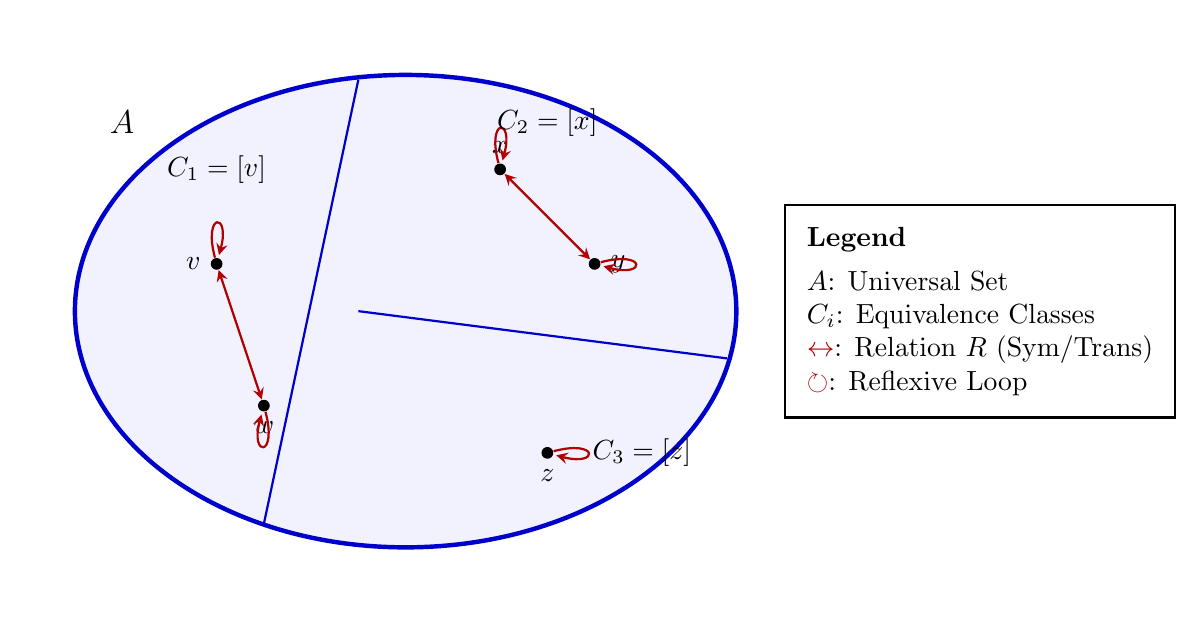
\begin{tikzpicture}[scale=1.2, >=stealth]
    % Background fill to ensure layering protocol
    \fill[white] (-4,-3) rectangle (6,3);
    
    % Draw the universal set A
    \draw[ultra thick, blue!80!black, fill=blue!5] (0,0) ellipse (3.5cm and 2.5cm);
    \node[black, font=\large\bfseries] at (-3, 2) {$A$};
    
    % Draw partition boundaries
    \draw[thick, blue!80!black] (-1.5, -2.25) -- (-0.5, 2.45);
    \draw[thick, blue!80!black] (-0.5, 0) -- (3.4, -0.5);
    
    % Nodes in Class 1
    \node[circle, fill=black, inner sep=1.5pt, label={[black]left:$v$}] (v) at (-2, 0.5) {};
    \node[circle, fill=black, inner sep=1.5pt, label={[black]below:$w$}] (w) at (-1.5, -1) {};
    \draw[<->, thick, red!70!black] (v) -- (w);
    \draw[->, thick, red!70!black] (v) edge[loop above] (v);
    \draw[->, thick, red!70!black] (w) edge[loop below] (w);
    \node[black, font=\bfseries] at (-2, 1.5) {$C_1 = [v]$};
    
    % Nodes in Class 2
    \node[circle, fill=black, inner sep=1.5pt, label={[black]above:$x$}] (x) at (1, 1.5) {};
    \node[circle, fill=black, inner sep=1.5pt, label={[black]right:$y$}] (y) at (2, 0.5) {};
    \draw[<->, thick, red!70!black] (x) -- (y);
    \draw[->, thick, red!70!black] (x) edge[loop above] (x);
    \draw[->, thick, red!70!black] (y) edge[loop right] (y);
    \node[black, font=\bfseries] at (1.5, 2) {$C_2 = [x]$};
    
    % Nodes in Class 3
    \node[circle, fill=black, inner sep=1.5pt, label={[black]below:$z$}] (z) at (1.5, -1.5) {};
    \draw[->, thick, red!70!black] (z) edge[loop right] (z);
    \node[black, font=\bfseries] at (2.5, -1.5) {$C_3 = [z]$};
    
    % Single-Node Multiline Legend using Anchor Pivot Strategy
    \node[align=left, anchor=west, inner sep=8pt, draw=black, fill=white, thick] at (4, 0) {
        \textbf{Legend} \\[4pt]
        $A$: Universal Set \\
        $C_i$: Equivalence Classes \\
        $\color{red!70!black}{\leftrightarrow}$: Relation $R$ (Sym/Trans) \\
        $\color{red!70!black}{\circlearrowright}$: Reflexive Loop
    };
\end{tikzpicture}
\end{center}
\vspace{1em}

\subsection{Heuristics \& Pitfalls}
\begin{itemize}
    \item \textbf{Heuristic (The "Difference" Trick):} If a relation is defined by an algebraic sum like $ax + by = k$, try to rewrite it as $a(x - y) + (a+b)y = k$. This often immediately reveals the underlying modular arithmetic (e.g., $x \equiv y \pmod{a+b}$).
    \item \textbf{Pitfall (Assuming Symmetry implies Reflexivity):} A classic fallacy is arguing: "If $x \mathrel{R} y$, then $y \mathrel{R} x$. By transitivity, $x \mathrel{R} x$, so it is reflexive." \textbf{Error:} This assumes there exists at least one $y$ such that $x \mathrel{R} y$. If an element $x$ is related to nothing, the premise fails, and reflexivity is violated.
    \item \textbf{Pitfall (Overlapping Partitions):} When defining equivalence classes manually, failing to ensure they are strictly disjoint. If $[a] \cap [b] \neq \emptyset$, they \textit{must} be the exact same set.
\end{itemize}

\newpage
\section{Conceptual Synthesis and The "Big Picture"}

\subsection{A) Thematic Connections}
The central theme of this topic is \textbf{Abstraction via Quotienting}. In mathematics, we often encounter sets that are too large or detailed for our specific analytical needs. Equivalence relations allow us to "mod out" the irrelevant details. By treating an entire equivalence class as a single point, we create a \textbf{Quotient Set} (denoted $A/R$). 
This unifies previous topics: modular arithmetic is simply the quotient set $\Z / \equiv_n$. Rational numbers $\Q$ are actually a quotient set of $\Z \times (\Z \setminus \{0\})$ under the equivalence relation $(a,b) \mathrel{R} (c,d) \iff ad = bc$.

\subsection{B) Forward and Backward Links}
\textbf{Backward Links:} This topic rigorously formalizes the intuitive set-theoretic operations (unions, intersections, partitions) learned in introductory logic. It provides the algebraic justification for why we can treat fractions like $1/2$ and $2/4$ as the "same" number.

\textbf{Forward Links:} Understanding equivalence classes is the absolute prerequisite for:
\begin{itemize}
    \item \textbf{Abstract Algebra:} The First Isomorphism Theorem relies entirely on mapping a group to its quotient group via the kernel (an equivalence class).
    \item \textbf{Topology:} Constructing complex shapes (like a Möbius strip or a Torus) is done by taking a flat space and defining an equivalence relation on its boundaries (gluing edges together).
    \item \textbf{Measure Theory \& Probability:} In advanced probability, random variables are formally defined as equivalence classes of measurable functions that agree "almost everywhere" (i.e., $f \mathrel{R} g \iff \Prob(f \neq g) = 0$).
\end{itemize}

\section{Abstract Real-World Modeling (AI, ML, \& Quant Finance)}

\subsection{A) Concrete Scenarios}
\begin{enumerate}
    \item \textbf{Reinforcement Learning (State Space Aggregation):} In Markov Decision Processes (MDPs) with massive state spaces (e.g., AlphaGo), computing the optimal policy is intractable. AI researchers use \textit{Bisimulation Equivalence Relations} to partition the state space. If two states yield the same immediate reward and have identical transition probabilities to all other equivalence classes, they are deemed equivalent. The AI then solves the MDP on the much smaller quotient space.
    \item \textbf{Quantitative Finance (Law of One Price):} In derivative pricing, an equivalence relation is defined on the space of all possible trading portfolios. Two portfolios are equivalent ($P_1 \mathrel{R} P_2$) if they yield the exact same payoff in every future state of the world. By the Law of One Price, equivalent portfolios must have the same current price, preventing arbitrage.
\end{enumerate}

\subsection{B) Model Problem Setup: Bisimulation in Stochastic MDPs}
Let us formalize the Reinforcement Learning scenario. 
Define a finite Markov Decision Process as a tuple $\mathcal{M} = (S, A, P, R)$, where $S$ is the state space, $A$ is the action space, $P(s' \mid s, a)$ is the transition probability measure, and $R(s, a)$ is the reward function.

We seek to define an equivalence relation $E \subseteq S \times S$ that partitions $S$ into a quotient space $S/E$. 
\begin{definition}[Stochastic Bisimulation]
An equivalence relation $E$ on $S$ is a bisimulation if, for all $(s_1, s_2) \in E$ and for all actions $a \in A$:
\begin{enumerate}
    \item $R(s_1, a) = R(s_2, a)$ (Reward Equivalence)
    \item For every equivalence class $C \in S/E$, $\sum_{s' \in C} P(s' \mid s_1, a) = \sum_{s' \in C} P(s' \mid s_2, a)$ (Transition Equivalence)
\end{enumerate}
\end{definition}
\textbf{Optimization Problem:} The goal in AI state abstraction is to find the \textit{coarsest} bisimulation relation $E^*$ (the one with the fewest equivalence classes) that satisfies these constraints. This reduces the Bellman Optimality Equation from dimension $|S|$ to dimension $|S/E^*|$, exponentially accelerating the convergence of algorithms like Q-Learning while guaranteeing zero loss in policy optimality.

\newpage
\section{Common Variations and Untested Concepts}

A standard advanced curriculum covers the \textbf{Canonical Projection Mapping}, a concept not explicitly tested in the provided homework but vital for algebraic structures.

\textbf{Concept: The Canonical Projection}
Given an equivalence relation $R$ on $A$, the quotient set is $A/R = \{ [a] \mid a \in A \}$. The canonical projection is the function $\pi: A \to A/R$ defined by $\pi(x) = [x]$. 

\textbf{Theorem Variation:} Prove that $\pi$ is surjective (onto), and that $\pi(x) = \pi(y) \iff x \mathrel{R} y$.

\textbf{Rigorous Proof:}
\textit{Surjectivity:} Let $Y \in A/R$. By definition of the quotient set, $Y$ is an equivalence class, so there exists some element $a \in A$ such that $Y = [a]$. Therefore, $\pi(a) = [a] = Y$. Since for every $Y \in A/R$ there exists an $a \in A$ mapping to it, $\pi$ is surjective.

\textit{Equivalence:} 
Assume $\pi(x) = \pi(y)$. By definition of the function, $[x] = [y]$. By Theorem 9.8, two equivalence classes are equal if and only if their representatives are related, so $x \mathrel{R} y$. 
Conversely, assume $x \mathrel{R} y$. By Theorem 9.8, $[x] = [y]$. Therefore, $\pi(x) = \pi(y)$.
$\blacksquare$

\section{Advanced Diagnostic Testing: "Find the Flaw"}

Below are five proofs containing subtle, critical logical flaws. Your task as the grader is to identify the error. (Solutions are provided at the end).

\textbf{Problem 1:} Let $R$ be a relation on $\R$ defined by $x \mathrel{R} y \iff |x - y| \le 1$. 
\textit{Flawed Proof of Equivalence:} 
1. Reflexive: $|x - x| = 0 \le 1$. True.
2. Symmetric: If $|x - y| \le 1$, then $|y - x| = |-(x - y)| = |x - y| \le 1$. True.
3. Transitive: If $|x - y| \le 1$ and $|y - z| \le 1$, then $x, y, z$ are all within a distance of 1 from each other, forming a bounded set. Thus $R$ is an equivalence relation.

\textbf{Problem 2:} Let $R$ and $S$ be equivalence relations on $A$. 
\textit{Flawed Proof that $R \cup S$ is an equivalence relation:}
Let $x, y, z \in A$. Assume $(x,y) \in R \cup S$ and $(y,z) \in R \cup S$. This means $(x,y)$ is in $R$ or $S$, and $(y,z)$ is in $R$ or $S$. Without loss of generality, assume they are both in $R$. Since $R$ is an equivalence relation, it is transitive, so $(x,z) \in R$. Since $(x,z) \in R$, it follows that $(x,z) \in R \cup S$. Thus, $R \cup S$ is transitive.

\textbf{Problem 3:} Let $R$ be a symmetric and transitive relation on $A$.
\textit{Flawed Proof of Reflexivity:}
Let $x \in A$. Choose some $y \in A$ such that $x \mathrel{R} y$. Since $R$ is symmetric, $x \mathrel{R} y \implies y \mathrel{R} x$. Since $R$ is transitive, $x \mathrel{R} y$ and $y \mathrel{R} x \implies x \mathrel{R} x$. Therefore, $R$ is reflexive and is an equivalence relation.

\textbf{Problem 4:} Let $A = \{1, 2, 3\}$. Define a partition $P = \{ \{1, 2\}, \{2, 3\} \}$.
\textit{Flawed Proof of Relation:}
By Theorem 9.12, every partition defines an equivalence relation. The relation is the union of the Cartesian products: $R = \{1,2\} \times \{1,2\} \cup \{2,3\} \times \{2,3\}$. Thus $R$ is an equivalence relation.

\textbf{Problem 5:} Prove that if $[a] = [b]$, then $a \mathrel{R} b$.
\textit{Flawed Proof:}
Assume $[a] = [b]$. By definition, $[a]$ contains all elements related to $a$, and $[b]$ contains all elements related to $b$. Since the classes are equal, $a$ and $b$ must be related to the exact same elements. Therefore, $a \mathrel{R} b$.

\vspace{1em}
\hrule
\vspace{1em}
\textbf{Solution Key (The Flaws Revealed):}
\begin{enumerate}
    \item \textbf{Flaw 1:} The transitivity argument is mathematically false. By the Triangle Inequality, $|x - z| \le |x - y| + |y - z| \le 1 + 1 = 2$. It does not guarantee $|x - z| \le 1$. (Counterexample: $x=0, y=1, z=2$).
    \item \textbf{Flaw 2:} The "Without loss of generality" assumption is a fatal logical error. It ignores the cross-case where $(x,y) \in R$ but $(y,z) \in S$. In this case, neither $R$ nor $S$ guarantees $(x,z)$ exists.
    \item \textbf{Flaw 3:} The proof assumes "Choose some $y \in A$ such that $x \mathrel{R} y$." There is no guarantee such a $y$ exists. If $x$ is related to nothing, the implication chain cannot even begin, and reflexivity fails.
    \item \textbf{Flaw 4:} $P$ is \textbf{not} a valid partition. A partition requires subsets to be pairwise disjoint. $\{1, 2\} \cap \{2, 3\} = \{2\} \neq \emptyset$. Theorem 9.12 cannot be applied.
    \item \textbf{Flaw 5:} The proof relies on vague English ("must be related") rather than rigorous set theory. The correct proof must use reflexivity: Since $R$ is reflexive, $a \in [a]$. Since $[a] = [b]$, it follows that $a \in [b]$. By definition of $[b]$, this means $a \mathrel{R} b$.
\end{enumerate}

\end{document}